{
{\sffamily Det er meget svært at kvantificere, hvorvidt det gyldne snit
bliver brugt i malerkunsten, men vi kan opstille nogle hypoteser for,
hvilke resultater vi vil forvente, hvis det gyldne snit bliver brugt.
De følgende hypoteser antager derfor den generelle opfattelse, at det
gyldne snit er specielt æstetisk tiltalende.
}

\begin{hypotese}
    Mere end $50\%$ af de analyserede malerier, har én eller flere
    regioner fundet i det gyldne snit.
    \label{hypo_binaer}
\end{hypotese}

\begin{hypotese}
    Antallet af regioner fundet i hvert af de fire snit tilknyttet snitratioen
    $\varPhi$, afviger ikke mere end $10\%$ fra hinanden.
    \label{hypo_fire_g_snit}
\end{hypotese}

\begin{hypotese}
    Mere end en tredjedel malerierne har et lærred, hvis
    dimensioner er lig $\varphi\pm2.4\%$.
    \label{hypo_golden_ractangle}
\end{hypotese}

\begin{hypotese}
    Antallet af fundne regioner i det gyldne snit er skarpt større, end
    antallet af regioner fundet i alle andre snit.
    \label{hypo_alle_andre_snit}
\end{hypotese}

\begin{hypotese}
    Antallet af regioner fundet i snitratioen $\varPhi$ er skarpt
    større, end antallet af regioner fundet i snitratioen $\frac{2}{3}$,
    pr. snit i snitratioen.
    \label{hypo_to_tredjedele}
\end{hypotese}

\begin{hypotese}
    Antallet af regioner fundet i det gyldne snit, er skarpt større, end
    antallet af regioner fundet det midterste snit.
    \label{hypo_midten}
\end{hypotese}

\begin{hypotese}
    Det gennemsnitlige antal fundne regioner i det gyldne snit pr.
    maleri, tidsperioder imellem, afviger med højst $10\%$.
    \label{hypo_tid}
\end{hypotese}

\begin{hypotese}
    Det gennemsnitlige antal fundne regioner i det gyldne snit pr.
    maleri, nationaliteter imellem, afviger med højst $10\%$.
    \label{hypo_nation}
\end{hypotese}

\begin{hypotese}
    Antallet af regioner fundet i snitratioen $\varPhi$, afviger ikke
    fra antallet af regioner fundet i snitratioen $\frac{2}{3}$, pr.
    snit, med mere end $15 \%$.
    \label{hypo_15p}
\end{hypotese}

Ovenstående hypoteser, er udarbejdet efter hvilke egenskaber, vi
forventer et maleri konstrueret efter det gyldne snit, har. Endvidere
antager vi, at det gyldne snit \emph{altid} har været at foretrække, på
tværs af landegrænser og kultur.

Hvis vi kun har malerier, som i alle henseender, er konstrueret efter det
gyldne snit, vil disse opfylde hypoteserne 1 -- 8. Dette vil betyde, at
regionerne i de gyldne snit dominerer, samt at brugen af det gyldne snit
ikke binder sig til nationalitet eller tidsperiode.

Kan en samling af malerier kun bekræfte nogle af hypoteserne fra 1 -- 8,
kan vi dog stadig sige noget om brugen af det gyldne snit. Hvis hypotese
3, som den eneste, ikke bliver opfyldt, kan vi stadig sige, at kunstnere
placerer de interessante regioner i maleriet efter det gyldne snit, men
ikke bruger det gyldne snit i valg af lærred.

Hypotese 5 og 9 er modsætninger. Nr. 5, hvis bekræftet, antyder at
kunstneren bevidst placerer interessante regioner i det gyldne snit. Nr.
9 derimod, antyder at snittet ved to tredjedele bliver brugt som
approksimation til det gyldne snit, og at de to snit bruges på lige fod.
Det vil sige at, \emph{hvis} det gyldne snit er specielt æstetisk
tiltalende, og \emph{hvis} to tredjedele bruges som approksimation til
det gyldne snit, så vil interessante regioner koncentrere sig om det
gyldne snit og snittet ved to tredjedele, og denne hypotese vil blive
bekræftet.

De tilladte afvigelser, er vores bedste bud på, hvornår det gyldne snit
ikke længere kan siges at være til stede i malerierne. Procentsatsen i
hypotese 3, er sat efter den fejlmargin vi fandt frem til i kapitel
\ref{chap_detektion}. De resterende procentsatser er valgt efter hvad
der virkede passende, da vi ingen tidligere har forsøgt at kvantificere
problemstillingen.

\subsection{Datasæt}
Det korpus, vi kører vores analyse på, består af billeder hentet fra
``The Web Gallery of Art''\cite{wgahu}, som er en online billededatabase, med
europæiske kunstartikler fra år 1001 -- 1900. I kunstartiklerne, hvor
det samlede antal er omkring 23.000, indgår møbler, kalkmalerier,
skulpturer, mosaikker og malerier, hvor sidstnævnte, vil være vores
fokus. Over halvdelen af disse kunstartikler står udstillet på museum.
Databasen blev oprettet i 1996, med det formål at præsentere kunst fra
renæssancen (ca.  14. -- 17.  århundrede), men blev senere udvidet, til
også at inkludere kunst fra andre perioder. Dette betyder, at
størstedelen af malerierne vi undersøger, er fra tidsperioden 1450 --
1650 og er malet af italienske kunstnere. Endvidere er langt de fleste
malerier klassificeret som religiøse.  Disse informationer er givet fra
WGA, men er også vedlagt i bilag \ref{appendix_grafer} som
grafer.

Vi må af ovenstående grunde forvente, at resultater, fra en analyse på
vores datasæt, vil være farvet af samlingen af malerier, og det derfor
kan være svært at drage nogen konklusioner for malerkunsten generelt, da
resultaterne vil være begrænset, til kun at gælde for et udsnit af
vestlig kultur. Endvidere findes der ingen nyere malerier i datasættet,
hvilket gør at vi ikke kan udtale os om nyere malerkunst.

Billederne, som suppleres fra databasen, er af høj kvalitet, men der er
visse problemer, som vi nævner nedenfor.

\begin{itemize}
    \item \textbf{Beskæring af billeder}\\
        Vi kan ikke vide os sikre på, om billederne i datasættet er
        ordentligt beskåret, hvilket f. eks. kan betyde, at noget af
        billedrammen kan være med i billedet. Dette kan muligvis volde
        lidt problemer med udtrækning af regioner, men hvad værre er, så
        gør det vores mål, for hvor det gyldne snit ligger, upræcist.
        Dette har vi dog taget højde for, i kraft af vores margin.
        Endelig er der inkluderet detaljebilleder af malerier i
        databasen, som er et udsnit af et givet maleri, således at
        målene for det gyldne snit ikke passer på billedet.
    \item \textbf{Forvrængning og perspektiv}\\
        Billederne af malerier er taget med et kamera, hvor linsen muligvis kan
        forvrænge billedet. Vi kan derfor have skæve linjer og tage
        forkerte beslutninger, for regioner, pga. dette. Endvidere kan
        billedet være taget skævt, således at billedet hælder til den
        ene side.
    \item \textbf{Opdelte malerier}\\
        Nogle store malerier kan være blevet opdelt i flere billeder, da
        databasen har det formål at vise malerierne på en computerskærm,
        hvor meget store billeder kan være svære at betragte. Dette
        betyder, at nogle billeder ikke viser hele maleriet, men blot er
        et udsnit, hvilket påvirker vores muligheder for at sige noget
        fornuftigt om det gyldne snit i maleriet.
\end{itemize}

Nogle stilarter, såsom kalkmalerier og tegninger, har gennem
udokumenterede afprøvninger, vist sig at være besværlige at analysere,
pga. meget svingende farvegengivelse. Endvidere, kan disse være billeder
af en hvælving i en kirke, som ikke egner sig til analyse for det gyldne
snit. Vi har derfor valgt kun at analysere malerier, kendetegnet ved at
de er beskrevet som ``painting'' fra WGA.

Alt det ovenstående vil påvirke resultaterne, ved analyse på vores
datasæt.

\subsection{Eksperimentsopstilling}
I afsnit \ref{chap_afproevning} er de optimale tærskelværdier fundet og
de er sat derefter.
Det er fordelagtigt at maksimere antallet af andre snit, da det giver et bedre grundlag for eksperimentet.  Afstanden
mellem to snit er begrænset af en margin defineret til at være
$2.4\%$, som beskrevet i kapitlet \ref{margin}.  Denne margin skal være tilstede på begge sider af
et snit, så derfor vil hvert snit fylde $(2.4*2)\%$.  Det maksimale
antal af snit på et billede må altså være $100/4.8=20.833$.
Med en margin på $2.4\%$ vil der være en strimmel på $0.1\%$ af
billedet, som ikke bliver brugt. Og mellem to marginer vil der derfor ligge en
strimmel på $0.2\%$. 

Den eneste undtagelse findes ved midten. I udregningen
\ref{resul_midt_udregning} ses først hvordan snittet til venstre for
midten findes, og derefter hvor lang afstanden er mellem de to snit.
\begin{equation}\label{resul_midt_udregningen}
    1-0.518 = 0.482
    0.518-0.482 = 0.036
\end{equation}
Der er altså en strimmel på $0.048-0.036 = 0.012 = 1.2\%$ af
billedet, hvor interessante regioner potentielt kunne blive talt to gange.
Dette er illustreret i figur \ref{resultat_fejl_midt}.
\begin{figure}[!h]
	\centering
	\fbox{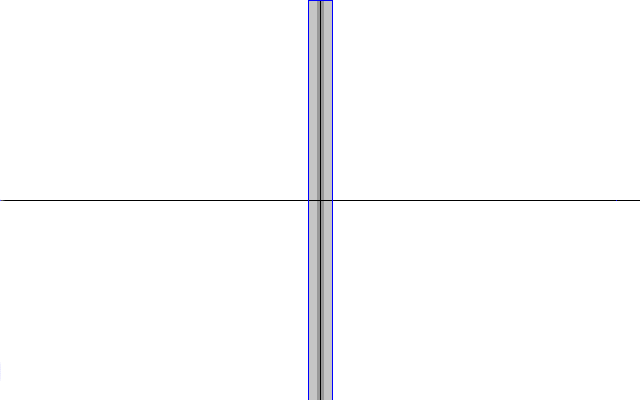
\includegraphics[scale=0.5]{afsnit/resultater/billeder/midt_strimmel}}
	\caption{Kollision mellem de to midterste snit,vist ved de to
	blå linjer.Midt er indikeret ved en sort linje, der ligger cirka
	midt i kollisionsområdet.}
	\label{resultat_fejl_midt}
\end{figure}

}
% vim: set tw=72 spell spelllang=da:
